
\section{Background and motivations}
\label{sec:background}

This section introduces the general outlines of state-of-the-art protocols in
charge of providing the random peer sampling which will be useful later
on. Also, it highlights the motivations of our approach.

\begin{asparadesc}
\item [WebRTC] is a protocol that allows real-time communication from browser
  to browser. It is able to establish a peer-to-peer connection, even with
  complex network settings such as firewall, proxies or Net Address Translation
  (NAT). Nevertheless, the connection establishment protocol differs from
  traditional setting: it uses a three-way handshake connection set up.  Thus,
  a subscription message must be
  \begin{inparaenum}[(1)]
  \item emitted at Peer $p$,
  \item accepted at Peer $q$,
  \item completed at Peer $p$.
  \end{inparaenum}
  Therefore, when a peer needs to establish a connection to another peer, a
  message must travel back and forth. One could use a dedicated server to
  establish the necessary dialog~\cite{peerjs}. However, this solution does not
  scale considering the fact that each peer in the network must dynamically
  create and remove connections over time. On the other hand, using the built
  network itself distributes the load of these connections establishment among
  the members.
\end{asparadesc}

\begin{asparadesc}
\item[Random peer sampling] protocols~\cite{jelasity2004peer} provide each peer
  with a partial view $\mathcal{P}$ of the network membership
  $\mathcal{N}$. They populate the partial views with peers chosen at random
  among $\mathcal{N}$ following a uniform distribution using local knowledge
  only. They aim to converge to a random graph, hence, providing connectedness,
  robustness and efficient epidemic spreading of messages. A wide variety of
  gossip-based protocols use random peer sampling (e.g. topology
  management~\cite{voulgaris2005epidemic,jelasity2009tman}).  Our \SCAMPLON{}
  protocol is inspired by two state-of-the-art approaches, namely \SCAMP{} and
  \CYCLON{}.
\end{asparadesc}

\begin{figure}
  \centering
  
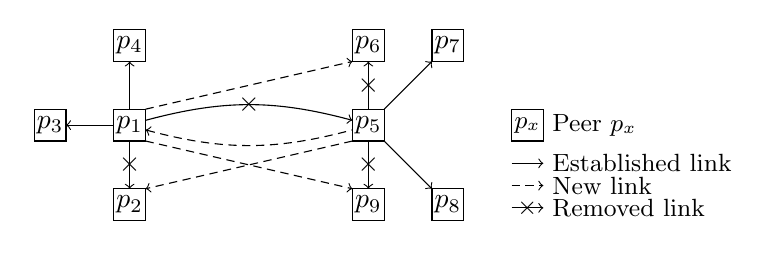
\begin{tikzpicture}[scale=1.15]
  
  \draw[fill=white] (0pt, 0pt) node{$p_1$} +(-5pt,-5pt) rectangle +(5pt,5pt);
  \draw[fill=white] ( 0pt,-25pt) node{$p_2$} +(-5pt,-5pt) rectangle +(5pt,5pt);
  \draw[fill=white] (-25pt,0pt) node{$p_3$} +(-5pt,-5pt) rectangle +(5pt,5pt);
  \draw[fill=white] ( 0pt,25pt) node{$p_4$} +(-5pt,-5pt) rectangle +(5pt,5pt);

  \draw[->] (-5pt, 0pt) -- (-20pt, 0pt); %% p1 -> p2
  \draw[->] ( 0pt, 5pt) -- (  0pt,20pt); %% p1 -> p3
  \draw[->] ( 0pt,-5pt) -- node{$\times$} (  0pt,-20pt); %% p1 -> p4
  
  \begin{scope}[shift={(75pt,0pt)}]
  \draw[fill=white] ( 0pt, 0pt) node{$p_5$} +(-5pt,-5pt) rectangle +(5pt,5pt);
  \draw[fill=white] (0pt,  25pt) node{$p_6$} +(-5pt,-5pt) rectangle +(5pt,5pt);
  \draw[fill=white] ( 25pt,25pt) node{$p_7$} +(-5pt,-5pt) rectangle +(5pt,5pt);
  \draw[fill=white] (25pt,-25pt) node{$p_8$} +(-5pt,-5pt) rectangle +(5pt,5pt);
  \draw[fill=white] (0pt, -25pt) node{$p_9$} +(-5pt,-5pt) rectangle +(5pt,5pt);

  \draw[->] ( 5pt, 5pt) -- ( 20pt, 20pt);
  \draw[->] ( 5pt, -5pt) -- ( 20pt,-20pt);
  \draw[->] ( 0pt, 5pt) -- node{$\times$} ( 0pt,20pt);
  \draw[->] ( 0pt,-5pt) -- node{$\times$} ( 0pt,-20pt);
  \end{scope}
  
  \draw[->, densely dashed] (5pt,5pt) -- (70pt,20pt); 
  \draw[->, densely dashed] (70pt,-5pt) -- (5pt,-20pt);
  \draw[->, densely dashed] ( 5pt,-5pt) -- (70pt,-20pt);
  \draw[->] (5pt, 1.5pt) to[out=15,in=165]
  node{$\times$} (70pt, 1.5pt);
  \draw[<-, densely dashed] (5pt, -1.5pt) to[out=-15,in=-165] (70pt,-1.5pt);

  \small 
  \begin{scope}[shift={(120pt,0pt)}]
    \draw[fill=white](5pt, 0pt)node{$p_x$}+(-5pt,-5pt) rectangle +(5pt,5pt);
    \draw (10pt,0pt) node[anchor=west]{Peer $p_x$};
    \draw[->](0pt, -12pt)--(10pt, -12pt) node[anchor=west]{Established link};
    \draw[->, densely dashed](0pt, -19pt)--(10pt, -19pt)
    node[anchor=west]{New link};
    \draw[->](0pt, -26pt)-- node{$\times$}(10pt, -26pt)
    node[anchor=west]{Removed link};
    
  \end{scope}
  
\end{tikzpicture}
  \caption{\label{fig:cyclonexample}Example of \CYCLON{}'s periodic exchange of
    partial views. For simplicity sake, we set $|\mathcal{P}|$ to $4$ and the
    peers involved in the exchange choose only $2$ neighbours among these
    $4$. Furthermore, while the network contains $9$ members, we only show the
    partial views of $p_1$ and $p_5$.  Peer $p_1$ initiates the view exchange
    with its oldest neighbour $p_5$, giving $\left\{p_1,\,p_2\right\}$
    (randomly chosen). On receipt, Peer $p_5$ establishes the connection to
    $p_1$ and $p_2$ and gives away its connection to $\left\{p_6,\,p_9\right\}$
    (randomly chosen).  On receipt of this latter, $p_1$ establishes the
    connection to Peer $p_6$ and Peer $p_9$. Altogether, we cut $4$ links to
    create $4$ other links only by using neighbour-to-neighbour interactions.}
\end{figure}

\begin{asparadesc}
\item [Cyclon]\cite{voulgaris2005cyclon} is a periodic random peer sampling
  protocol which updates its partial view every interval of time. The partial
  view has a fixed-size set at start. In this view, each neighbor is
  associated with an age incremented at each cycle. To update its partial view,
  \CYCLON{} exchanges a subset of its partial view with one of its neighbor
  chosen using the age.  Assuming a well chosen $|\mathcal{P}|$, \CYCLON{}
  quickly converges to a random graph and quickly withdraws crashed/left peers.
  Figure~\ref{fig:cyclonexample} depicts the periodic exchanges of
  \CYCLON{}. In particular, we can see that peers only communicate in their
  direct neighborhood to renew the connections.

  In the WebRTC context, each connection matters. Hence, we cannot afford
  oversized partial views like in \CYCLON{}. For instance, considering an
  application usable by small or large groups of users indifferently, \CYCLON{}
  will overestimate to adapt to the largest groups. While this is indeed
  required for these latter, the small groups of users will suffer of increased
  traffic (oversized partial views maintenance, increased redundancy during the
  broadcast of messages). If the group is small enough, the graph could be
  fully connected which is highly undesirable.
\end{asparadesc}

\begin{figure}
  \centering
  
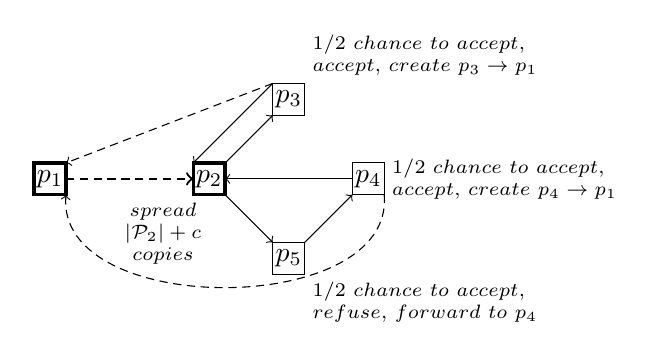
\begin{tikzpicture}[scale=1.15]
  
  \draw[fill=white, very thick] (0pt, 0pt)
  node{$p_1$} +(-5pt,-5pt) rectangle +(5pt,5pt);

  \begin{scope}[shift={(75pt,0pt)}]
  \draw[fill=white, very thick]
  (-25pt, 0pt) node{$p_2$} +(-5pt,-5pt) rectangle +(5pt,5pt);
  \draw[fill=white] (0pt,  25pt) node{$p_3$} +(-5pt,-5pt) rectangle +(5pt,5pt);
  \draw[fill=white] ( 25pt, 0pt) node{$p_4$} +(-5pt,-5pt) rectangle +(5pt,5pt);
  \draw[fill=white] (0pt, -25pt) node{$p_5$} +(-5pt,-5pt) rectangle +(5pt,5pt);


  \draw[->] (-20pt, 5pt) -- (-5pt, 20pt); 
  \draw[->] (-20pt,-5pt) -- (-5pt,-20pt); 
  \draw[->] ( 5pt,-20pt) -- (20pt, -5pt); 
  \draw[->] (20pt,  0pt) -- (-20pt, 0pt); 
  \draw[->] (-5pt, 30pt) -- (-30pt, 5pt); 

  \draw[->, thick, densely dashed] (-70pt, 0pt) -- (-30pt, 0pt); 
  \draw[->, densely dashed] (-5pt, 30pt) -- (-70pt, 5pt); 
  \draw[->, densely dashed] (30pt, -5pt)to[out=-85,in=-95](-70pt,-5pt);

  \scriptsize
  \draw (-25pt,-5pt) node[align=center,anchor=north east]
  {$spread$\\$|\mathcal{P}_2|+c$\\$copies$};
  \draw (5pt,-30pt) node[align=left,anchor=north west]
  {$1/2$ $chance$ $to$ $accept,$\\$refuse,$ $forward$ $to$ $p_4$};
  \draw (5pt, 30pt) node[align=left,anchor=south west]
  {$1/2$ $chance$ $to$ $accept,$\\$accept,$ $create$ $p_3 \rightarrow p_1$};
  \draw (30pt, 0pt) node[align=left,anchor=west]
  {$1/2$ $chance$ $to$ $accept,$\\$accept,$ $create$ $p_4 \rightarrow p_1$};
  \end{scope}
  
%%  \small
%%  \begin{scope}[shift={(130pt,0pt)}]
%%    \draw[fill=white](5pt, 0pt)node{$p_x$}+(-5pt,-5pt) rectangle +(5pt,5pt);
%%    \draw (10pt,0pt) node[anchor=west]{Peer $p_x$};
%%    \draw[->](0pt, -12pt)--(10pt, -12pt) node[anchor=west]{Established link};
%%    \draw[->, densely dashed](0pt, -19pt)--(10pt, -19pt)
%%    node[anchor=west]{New link};
%%    
%%  \end{scope}
  
\end{tikzpicture}
  \caption{\label{fig:scampexample} \SCAMP{}'s joining protocol on a small
    network with an identical legend to Figure~\ref{fig:cyclonexample}. Peer
    $p_1$ wants to join $p_2$'s network composed of $p_2$, $p_3$, $p_4$, and
    $p_5$. Let $\mathcal{P}_x$ denotes the partial view of Peer $p_x$. Peer
    $p_1$ establishes a connection to $p_2$. Then $p_2$ copies
    $|\mathcal{P}_2|$-times the new subscription and sends one to each
    neighbour. To handle possible failures, $c$ additional copies (here $0$ for
    simplicity sake), are sent to random neighbours. Then, each peer $p_x$ has
    a probability of $1\over{|\mathcal{P}_x|+1}$ to accept the forwarded
    subscription, hence, to establish a connection to reach $p_1$. Otherwise,
    the peer forwards it to another peer in $\mathcal{P}$ at random. Here,
    $p_3$ accepts the subscription, $p_5$ forwards it to $p4$, and the latter
    accepts it. The resulting graph is connected.}
\end{figure}

\begin{asparadesc}
\item [Scamp]\cite{ganesh2001scamp,ganesh2003peer} stands for SCalable
  Membership Protocol. This protocol links each membership event with an
  appropriate reaction.  The most important event is the joining event which
  creates a logarithmically increasing number of connections compared to the
  total network size.  Figure~\ref{fig:scampexample} depicts the joining
  protocol of \SCAMP{}. As we can see, the resulting graph is
  connected. However, the last peer $p_1$ only has one neighbor in its partial
  view, meaning that if $p_2$ crashes, $p_1$ cannot send messages to the
  network any more. To avoid that, a periodic re-subscription balances the
  neighborhood of the peers over time. Thus, the network converges to a random
  graph.

  In the WebRTC context, the issue of \SCAMP{} lies in the fact that the
  subscription mechanism can create connections several hops away from its
  origin (cf. Figure~\ref{fig:handshakeexample}). Unfortunately each of these
  hops is an opportunity of failure. Let $P_f$ the probability of either the
  peer or the link between the latter and the next peer crashes/disconnects
  when it holds the subscription, without possible recovery. Let $P_E$ the
  probability that a connection establishment cannot be completed. Without
  three-way handshake, $P_E$ is straightforward:
  \begin{equation} P_{E,\,1way}^{SCAMP}=1-(1- P_f)^{k+1} \end{equation} where
  $k$ is the number of hops before the acceptance of the subscription, i.e.,
  there are $2$ hops at least. Indeed, the first peer cannot directly accept
  the subscription. On the other hand, in the handshaking context, the
  subscription must travel back to its origin in order to be completed. As
  consequence, when a subscription travels through a peer or a link, they are
  not allowed to fail until the subscription travels back. Thus, we obtain:
  \begin{align} P_{E,\,3way}^{SCAMP} &=1 - ((1-P_f)^{2(k+1)} (1-P_f)^{2k}
                                       \ldots (1-P_f)^2) \nonumber \\
                                     &=1-(1-P_f)^{k^2+3k+2}
  \end{align}
  The complexity class of the \SCAMP{} failure rate under three-way handshake
  increases. Thus, it does not scale in number of peers any more.
\end{asparadesc}

\begin{figure}
  \centering
  
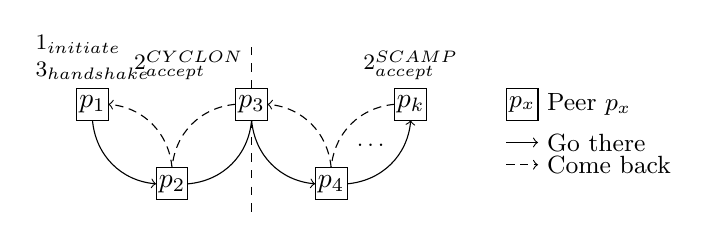
\begin{tikzpicture}[scale=1.15]

  \footnotesize
  \draw (0pt,5pt)node[align=left,anchor=south]{$1_{initiate}$\\
    $3_{handshake}$};
  \draw (50pt, 5pt)node[anchor=south east]{$2_{accept}^{CYCLON}$};
  \draw (100pt,5pt)node[anchor=south]{$2_{accept}^{SCAMP}$};
  \draw (88pt, -13pt)node{\ldots};

  \draw[dashed](50pt,-5pt)--(50pt,-35pt);
  \draw[dashed](50pt, 5pt)--(50pt, 20pt);

  \normalsize
  \draw[fill=white] (0pt, 0pt) node{$p_1$} +(-5pt,-5pt) rectangle +(5pt,5pt);
  \draw[fill=white] (25pt,-25pt) node{$p_2$} +(-5pt,-5pt) rectangle +(5pt,5pt);
  \draw[fill=white] (50pt, 0pt) node{$p_3$} +(-5pt,-5pt) rectangle +(5pt,5pt);
  \draw[fill=white] (75pt,-25pt) node{$p_4$} +(-5pt,-5pt) rectangle +(5pt,5pt);
  \draw[fill=white] (100pt, 0pt) node{$p_k$} +(-5pt,-5pt) rectangle +(5pt,5pt);


  \draw[->] ( 0pt,-5pt) to[out=-85,in=175] (20pt,-25pt);
  \draw[->, densely dashed] (25pt, -20pt) to[out=95,in=-5] ( 5pt, 0pt);
  \draw     ( 30pt, -25pt) to[out=5,in=-95] (50pt,-5pt);
  \draw[densely dashed] ( 45pt, 0pt) to[out=185,in=85] (25pt, -20pt);
  \draw[->] (50pt, -5pt) to[out=-85,in=175] (70pt,-25pt);
  \draw[->, densely dashed] (75pt, -20pt) to[out=95,in=-5] (55pt,0pt);
  \draw[->] (80pt, -25pt) to[out=5pt,in=-95] (100pt,-5pt);
  \draw[densely dashed] (95pt, 0pt) to[out=185,in=85] (75pt, -20pt);
%%  \draw[->, densely dashed] (-70pt, 0pt) -- (-30pt, 0pt); %% u1 -> u4
%%  \draw[->, densely dashed] (-5pt, 30pt) -- (-70pt, 5pt); %% u3 -> u1
%%  \draw[->, densely dashed] (30pt, -5pt) to[out=-85,in=-95](-70pt,-5pt);%%u5 u1

  \small 
  \begin{scope}[shift={(130pt,0pt)}]
    \draw[fill=white](5pt, 0pt)node{$p_x$}+(-5pt,-5pt) rectangle +(5pt,5pt);
    \draw (10pt,0pt) node[anchor=west]{Peer $p_x$};
    \draw[->](0pt, -12pt)--(10pt, -12pt) node[anchor=west]{Go there};
    \draw[->, densely dashed](0pt, -19pt)--(10pt, -19pt)
    node[anchor=west]{Come back};    
  \end{scope}
  
\end{tikzpicture}
  \caption{\label{fig:handshakeexample}Handshaking differences of \CYCLON{} and
    \SCAMP{}. While subscriptions travel from $p_1$ to $p_3$ using one
    intermediate in \CYCLON{}, the subscriptions travel from $p_1$ to $p_k$ in
    \SCAMP{}. This difference change the complexity of the two approaches. In
    particular, the failure probability is much more important in
    \SCAMP{}. Indeed, links and peers, once employed, must be kept alive until
    the subscriptions travel back. Otherwise, the handshaking cannot be
    completed.}
\end{figure}

\begin{problem}
  Let $t$ be an arbitrary time frame, let $\mathcal{N}^t$ be the network
  membership at that given time $t$ and let $\mathcal{P}_x^t$ be the partial view of peer $p_x \in \mathcal{N}^t$. 
  A random peer sampling, especially when three-way handshaking is involved, should provide the following best-case properties:
  \begin{center}
    Partial view size: \hfill $\forall p_x^t, |\mathcal{P}_x^t| = \Theta (\text{ln}\, |\mathcal{N}^t|)$
  \end{center}
  \begin{center}
    Time complexity of a connection: \hfill $O(1)$
  \end{center}
  \begin{center}
    Convergence speed: \hfill $\Omega(\exp \, t^{-1})$
  \end{center}
\end{problem}

Unfortunately, while both approaches converge exponentially fast to a random
graph, each of them fails either on the partial view size requirement
(i.e. \CYCLON{}) or the time complexity of connection establishment
(i.e. \SCAMPLON{}). Knowingly, we would like the best of the aforementioned
approaches in order to answer to the problem statement. Ultimately, it would
allow gossiping on top of WebRTC. Hence, it would open the gate to a wide
variety of distributed and decentralized applications requiring a scalable
broadcast.

%%% Local Variables:
%%% mode: latex
%%% TeX-master: "../paper"
%%% End:
